\documentclass{ximera}

% These macros are automatically generated from the "macros"
% XML element.  Make permanent edits there.
%
% History
%   2004/01/01  Initiated for FCLA, evolved from there
%   2006/09/17  Converted  _, ^  to \sb, \sp for TeX4ht
%   2014/02/01  Updated for MathBook XML projects
%               Obsolete in FCLA: \codeindent, \computerfont, \define
%               Change: MathJax wants \lt, so replaced by \lteval
%   2014/02/22  New: \orderof, \reals, \per
%   2015/08/16  Incorporated into MathBook XML version of FCLA
%
%%%%%%%%%%%%%%%%%%%%%
%
%     Conveniences
%
%%%%%%%%%%%%%%%%%%%%%
%
%  Order of (asymptotically limit of fraction is 1)
%  Usage: \orderof{some function}
%
\newcommand{\orderof}[1]{\sim #1}
%
%  Integers
%  Usage:  \Z
\newcommand{\Z}{\mathbb{Z}}
%
%  Real numbers, as set of scalars
%  Usage:  \reals
\newcommand{\reals}{\mathbb{R}}
%
%  n-space over real field
%  Usage: \complex{integer-dimension}
\newcommand{\real}[1]{\mathbb{R}^{#1}}
%
%  Complex numbers, as set of scalars
%  Usage:  \complexes
\newcommand{\complexes}{\mathbb{C}}
%
%  n-space over complex field
%  Usage: \complex{integer-dimension}
\newcommand{\complex}[1]{\mathbb{C}^{#1}}
\newcommand{\CC}{\mathbb{C}}
%
%  Complex conjugation (scalar, vector, matrix)
%  Usage: \conjugate{object}
\newcommand{\conjugate}[1]{\overline{#1}}
%
%  Complex number modulus
%  Usage: \modulus{a+bi}
%  Presumes math mode
\newcommand{\modulus}[1]{\left\lvert#1\right\rvert}
%
%  Zero vector
%  Usage: \zerovector
\newcommand{\zerovector}{\vect{0}}
%
%  Zero matrix
%  Usage: \zeromatrix, use a subscript when size is important
\newcommand{\zeromatrix}{\mathcal{O}}
%
%  Inner product (brackets, not quadratic form)
%  Usage: \innerproduct{a-vector}{a-vector}
\newcommand{\innerproduct}[2]{\left\langle#1,\,#2\right\rangle}
%
%  Norm of a vector
%  Usage: \norm{a-vector}
\newcommand{\norm}[1]{\left\lVert#1\right\rVert}
%
%  Dimension
%  Usage: \dimension{vector-space-letter}
\newcommand{\dimension}[1]{\dim\left(#1\right)}
%
%  Nullity
%  Usage: \nullity{matrix-or-lintrans-letter}
\newcommand{\nullity}[1]{n\left(#1\right)}
%
%  Rank
%  Usage: \rank{matrix-or-lintrans-letter}
\newcommand{\rank}[1]{r\left(#1\right)}
%
%  Direct sum
%  Usage: \ds between a couple of subspaces
%
\newcommand{\ds}{\oplus}
%
%  Determinant of a matrix (functional)
%  Usage: \detname{A}
\newcommand{\detname}[1]{\det\left(#1\right)}
%
%  Determinant of a matrix (vertical bars)
%  Usage: \detbars{A}
\newcommand{\detbars}[1]{\left\lvert#1\right\rvert}
%
%  Trace of a Matrix
%  Usage: \trace{matrix name}
\newcommand{\trace}[1]{t\left(#1\right)}
%
%  Square Root of a Matrix
%  Usage: \sr{a-matrix}
\newcommand{\sr}[1]{#1^{1/2}}
%
%%%%%%%%%%%%%%%%%%%%%
%
%     Subspace Constructions
%
%%%%%%%%%%%%%%%%%%%%%
%
%  Span of a set of vectors
%  \span and \sp are used by TeX for other things
%  Usage: \spn{set-of-vectors}
\newcommand{\spn}[1]{\left\langle#1\right\rangle}
%
%  Null space of a matrix
%  Usage:  \nsp{A}
\newcommand{\nsp}[1]{\mathcal{N}\!\left(#1\right)}
%
%  Column space of a matrix
%  Usage:  \csp{A}
\newcommand{\csp}[1]{\mathcal{C}\!\left(#1\right)}
%
%  Row space of a matrix
%  Usage:  \rsp{A}
\newcommand{\rsp}[1]{\mathcal{R}\!\left(#1\right)}
%
%  Left null space of a matrix
%  Usage:  \lns{A}
\newcommand{\lns}[1]{\mathcal{L}\!\left(#1\right)}
%
%  Orthogonal complement of a vector space
%  Avoiding TeX's \perp
%  Usage:  \per{A}
\newcommand{\per}[1]{#1^\perp}
%
%%%%%%%%%%%%%%%%%%%%%
%
%     Systems of Equations
%
%%%%%%%%%%%%%%%%%%%%%
%
%  In-line form of an augmented matrix for a system of equations
%  Usage: \augmented{coefficient-matrix}{constant-vector}
\newcommand{\augmented}[2]{\left\lbrack\left.#1\,\right\rvert\,#2\right\rbrack}
%
%  Notation for a linear system before introducing matrix multiplication
%  Usage: \linearsystem{coefficient-matrix}{constant-vector}
\newcommand{\linearsystem}[2]{\mathcal{LS}\!\left(#1,\,#2\right)}
%
%  Notation for a homogenous system before introducing matrix multiplication
%  Usage: \homosystem{coefficient-matrix}
\newcommand{\homosystem}[1]{\linearsystem{#1}{\zerovector}}
%
%%%%%%%%%%%%%%%%%%%%%
%
%     Row Operations, Echelon Form
%
%%%%%%%%%%%%%%%%%%%%%
%
% Row operations on matrices
%
% Three commands to shorten up descriptions of gaussian elimination
%
% Usage: \rowopswap{row-i}{row-j}
% Usage: \rowopmult{scalar}{row-i}
% Usage: \rowopadd{scalar}{row-multiplied}{row-added-to}
\newcommand{\rowopswap}[2]{R_{#1}\leftrightarrow R_{#2}}
\newcommand{\rowopmult}[2]{#1R_{#2}}
\newcommand{\rowopadd}[3]{#1R_{#2}+R_{#3}}
%
% Mark leading 1's in echelon form with fbox
% Usage: \leading{a-1-usually}
\newcommand{\leading}[1]{\fbox{#1}}
%
%  Row-reduce arrow
%  Usage:  \rref inbetween a matrix and its reduced row-echelon form
\newcommand{\rref}{\xrightarrow{\text{RREF}}}
%
%  Elementary Matrices
%  Usage: \elemswap{subscript}{subscript}
%  Usage: \elemmult{scalar}{subscript}
%  Usage: \elemadd{scalar}{subscript-mult}{subscript-target}
%
\newcommand{\elemswap}[2]{E_{#1,#2}}
\newcommand{\elemmult}[2]{E_{#2}\left(#1\right)}
\newcommand{\elemadd}[3]{E_{#2,#3}\left(#1\right)}
%
%%%%%%%%%%%%%%%%%%%%%
%
%     2-D Constructions (Lists, Vectors, Matrices)
%
%%%%%%%%%%%%%%%%%%%%%
%
%  A list of scalars of generic length
%  Usage:  \scalarlist{scalar letter}{terminal subscript}
\newcommand{\scalarlist}[2]{{#1}_{1},\,{#1}_{2},\,{#1}_{3},\,\ldots,\,{#1}_{#2}}
%
%  Vector styling, bold (or use wiggles, arrows, whatever)
%  Subscripts go outside this construction
%  Usage: \vect{a symbol to use as a vector}
%  Have to already be in math mode
%
\newcommand{\vect}[1]{\mathbf{#1}}
%
%  A column vector
%  Usage: \colvector{list-delimited-by-\\}
%
\newcommand{\colvector}[1]{\begin{bmatrix}#1\end{bmatrix}}
%
%  A generic vector with components
%  Usage: \vectorcomponents{component-letter}{final-subscript}
\newcommand{\vectorcomponents}[2]{\colvector{#1_{1}\\#1_{2}\\#1_{3}\\\vdots\\#1_{#2}}}
%
%  A list of vectors of generic length
%  Usage:  \vectorlist{vector letter}{terminal subscript}
\newcommand{\vectorlist}[2]{\vect{#1}_{1},\,\vect{#1}_{2},\,\vect{#1}_{3},\,\ldots,\,\vect{#1}_{#2}}
%
%  Vector entries, entry i of vector v
%  (vector-expession still needs \vect, etc.)
%  Usage:  \vectorentry{vector-expression}{single-subscript}
\newcommand{\vectorentry}[2]{\left\lbrack#1\right\rbrack_{#2}}
%
%  Matrix entries, entry i,j of matrix A
%  Usage:  \matrixentry{matrix-expression}{paired-subscripts}
%
\newcommand{\matrixentry}[2]{\left\lbrack#1\right\rbrack_{#2}}
%
%  A generic linear combination
%  Usage:  \lincombo{scalar letter}{vector letter}{terminal subscript}
\newcommand{\lincombo}[3]{#1_{1}\vect{#2}_{1}+#1_{2}\vect{#2}_{2}+#1_{3}\vect{#2}_{3}+\cdots +#1_{#3}\vect{#2}_{#3}}
%
%  Matrix, column by column, as vectors
%  Usage:  \matrixcolumns{matrix letter}{terminal subscript}
\newcommand{\matrixcolumns}[2]{\left\lbrack\vect{#1}_{1}|\vect{#1}_{2}|\vect{#1}_{3}|\ldots|\vect{#1}_{#2}\right\rbrack}
%
%%%%%%%%%%%%%%%%%%%%%
%
%     Special Matrices
%
%%%%%%%%%%%%%%%%%%%%%
%
%  Transpose of a matrix
%  Usage:  \transpose{A}
\newcommand{\transpose}[1]{#1^{t}}
%
%  Inverse of a matrix
%  Usage:  \inverse{A}
\newcommand{\inverse}[1]{#1^{-1}}
%
%  Submatrix (for minors, determinants)
%  Usage: \submatrix{matrix-name}{delete-row}{delete-col}
\newcommand{\submatrix}[3]{#1\left(#2|#3\right)}
%
%  Adjoint of a matrix (twice)
%  This macro is a convenience to call \transpose and \conjugate properly
%  It shouldn't need to be modified (or mathematical meanings will change)
%  Usage:  \adj{A}
\newcommand{\adj}[1]{\transpose{\left(\conjugate{#1}\right)}}
%
%  This macro controls the symbol used for the adjoint
%  It can be edited to taste
%  Usage:  \adjoint{A}
\newcommand{\adjoint}[1]{#1^\ast}
%
%%%%%%%%%%%%%%%%%%%%%
%
%     Sets
%
%%%%%%%%%%%%%%%%%%%%%
%
%  A convenience for simple sets
%  Usage:  \set{list of element}
\newcommand{\set}[1]{\left\{#1\right\}}
%
%  Sets with vertical bar, "such that", sized for objects, not condition
%  Usage:  \setparts{objects}{condition}
%
%%\newcommand{\setparts}[2]{\left\{ #1\mid#2\right\}}
%%\newcommand{\setparts}[2]{\left\{\left. #1\right\rvert#2\right\}}
\newcommand{\setparts}[2]{\left\lbrace#1\,\middle|\,#2\right\rbrace}
%
%  Set Cardinality
%  Usage:  \card{a-set-letter}
\newcommand{\card}[1]{\left\lvert#1\right\rvert}
%
%  Set Union
%  Use \cup
%
%  Set Intersection
%  Use \cap
%
%  Set Complement
%  Usage:  \setcomplement{a-set-letter}
\newcommand{\setcomplement}[1]{\overline{#1}}
%
%%%%%%%%%%%%%%%%%%%%%
%
%     Eigenvalues and Eigenspaces
%
%%%%%%%%%%%%%%%%%%%%%
%
%  Characteristic polynomial
%  Usage: \charpoly{matrix-letter}{variable-letter}
\newcommand{\charpoly}[2]{p_{#1}\left(#2\right)}
%
%  Eigenspace
%  Usage: \eigenspace{matrix-letter}{eigenvalue-letter}
\newcommand{\eigenspace}[2]{\mathcal{E}_{#1}\left(#2\right)}
%
%  2013/10/03 Including ampersands is problematic here, 
%  think about fixes later
%  2014/02/22 Limited testing, seems &amp; is fine for HTML and LaTeX
%  2016-07-20 only employed in Archetypes, MBX has gather/align override
%  Eigensystem (presumes wrapped in an mrow within md)
%  Usage: \eigensystem{matrixletter}{eigenvalue}{list of basis vectors}
\newcommand{\eigensystem}[3]{\lambda&amp;=#2&amp;\eigenspace{#1}{#2}&amp;=\spn{\set{#3}}} 
%
%  Generalized Eigenspace
%  Usage: \geneigenspace{lin-trans-letter}{eigenvalue-letter}
\newcommand{\geneigenspace}[2]{\mathcal{G}_{#1}\left(#2\right)}
%
%  Algebraic multiplicty
%  Usage: \algmult{matrix-letter}{eigenvalue-letter}
\newcommand{\algmult}[2]{\alpha_{#1}\left(#2\right)}
%
%  Geometric multiplicty
%  Usage: \geomult{matrix-letter}{eigenvalue-letter}
\newcommand{\geomult}[2]{\gamma_{#1}\left(#2\right)}
%
%  Index (of eigenvalue)
%  Usage: \indx{matrix-letter}{eigenvalue-letter}
\newcommand{\indx}[2]{\iota_{#1}\left(#2\right)}
%
%%%%%%%%%%%%%%%%%%%%%
%
%     Linear Transformations
%
%%%%%%%%%%%%%%%%%%%%%
%
%  MathJax defines \lt to ease XML confusion
%
%  Linear transformation definition
%  Usage: \ltdefn{name-letter}{domain}{range}
\newcommand{\ltdefn}[3]{#1\colon #2\rightarrow#3}
%
%  Linear transformation evaluation
%  Usage: \lteval{name-letter}{input}
%  Replaces old \lt desired by MathJax
\newcommand{\lteval}[2]{#1\left(#2\right)}
%
% Linear transformation inverse
%  Usage: \ltinverse{name-letter}
\newcommand{\ltinverse}[1]{#1^{-1}}
%
%  Linear transformation restriction
%  Usage: \restrict{name-letter}{subspace-letter}
\newcommand{\restrict}[2]{{#1}|_{#2}}
%
%  Linear transformation preimage
%  Usage: \preimage{name-letter}{codomain-element}
\newcommand{\preimage}[2]{#1^{-1}\left(#2\right)}
%
%  Range of a linear transformation
%  TeX uses \range for something else
%  Usage:  \rng{T}
\newcommand{\rng}[1]{\mathcal{R}\!\left(#1\right)}
%
%  Kernel of a linear transformation
%  TeX uses \ker to do something different
%  Usage:  \krn{T}
\newcommand{\krn}[1]{\mathcal{K}\!\left(#1\right)}
%
%  Linear transformation composition
%  Usage: \compose{function-name}{function-name}
\newcommand{\compose}[2]{{#1}\circ{#2}}
%
%  Vector space of linear transformations
%  Usage: \vslt{domains}{codomains}
%  Presumes math mode
\newcommand{\vslt}[2]{\mathcal{LT}\left(#1,\,#2\right)}
%
%%%%%%%%%%%%%%%%%%%%%
%
%     Vector and Matrix Representations
%
%%%%%%%%%%%%%%%%%%%%%
%
%  Isomorphism symbol
%  Usage: \isomorphic
\newcommand{\isomorphic}{\cong}
%
%  Similarity
%  Usage: \similar{inner-matrix}{outer-invertible-matrix}
%  Rearranging this will not "fix" all desired changes throughout
%
\newcommand{\similar}[2]{\inverse{#2}#1#2}
%
%  Vector representation function name
%  Usage: \vectrepname{basis-letter}
\newcommand{\vectrepname}[1]{\rho_{#1}}
%
%  Vector representation output
%  Usage: \vectrep{basis-letter}{input}
\newcommand{\vectrep}[2]{\lteval{\vectrepname{#1}}{#2}}
%
%  Vector representation inverse function name
%  (Added later, not used consistently in FCLA)
%  Usage: \vectrepinvname{basis-letter}
\newcommand{\vectrepinvname}[1]{\ltinverse{\vectrepname{#1}}}
%
%  Vector representation inverse output
%  Usage: \vectrepinv{basis-letter}{input}
\newcommand{\vectrepinv}[2]{\lteval{\ltinverse{\vectrepname{#1}}}{#2}}
%
%  Matrix representation
%  Usage: \matrixrep{transformation-letter}{domain-basis-letter}{codomain-basis-letter}
\newcommand{\matrixrep}[3]{M^{#1}_{#2,#3}}
%
%  Matrix representation column-by-colum
%  2016-07-20 only employed once?
%  Usage: \matrixrepcolumns{transformation-letter}{codomain-basis-letter}{codomain-basis-vector-letter}{final-index}
\newcommand{\matrixrepcolumns}[4]{\left\lbrack \left.\vectrep{#2}{\lteval{#1}{\vect{#3}_{1}}}\right|\left.\vectrep{#2}{\lteval{#1}{\vect{#3}_{2}}}\right|\left.\vectrep{#2}{\lteval{#1}{\vect{#3}_{3}}}\right|\ldots\left|\vectrep{#2}{\lteval{#1}{\vect{#3}_{#4}}}\right.\right\rbrack}
%
%  Change of basis matrix
%  Usage: \cbm{domain-basis-letter}{codomain-basis-letter}
\newcommand{\cbm}[2]{C_{#1,#2}}
%
%%%%%%%%%%%%%%%%%%%%%
%
%     Canonical Forms
%
%%%%%%%%%%%%%%%%%%%%%
%
%  Jordan blocks
%  Usage: \jordan{size}{diagonal-element}
\newcommand{\jordan}[2]{J_{#1}\left(#2\right)}
%
%%%%%%%%%%%%%%%%%%%%%
%
%     Hadamard Matrices
%     Contributed by Elizabeth Million
%
%%%%%%%%%%%%%%%%%%%%%
%
%  Hadamard Product
%  Usage: \hadamard{a-matrix}{a-matrix}
\newcommand{\hadamard}[2]{#1\circ #2}
%
%  Hadamard identity matrix
%  Usage: \hadamardidentity{paired-subscripts-size-of-matrix}
\newcommand{\hadamardidentity}[1]{J_{#1}}
%
%  Hadamard inverse matrix
%  Usage: \hadamardinverse{matrix-expression}
\newcommand{\hadamardinverse}[1]{\widehat{#1}}

\newcommand{\definedTerm}[1]{\textbf{#1}}
\newcommand{\dfn}[1]{\textbf{#1}}

\newcommand{\wt}{\widetilde}
\newcommand{\ov}{\overline}
\newcommand{\inj}{\rightarrowtail}
\newcommand{\surj}{\twoheadrightarrow}
\newcommand{\harpoon}{\overset{\rightharpoonup}}

\newenvironment{amatrix}[1]{%
  \left[\begin{array}{@{}*{#1}{c}|c@{}}
}{%
  \end{array}\right]
}


\title{Kernel of a Linear Transformation}

\begin{document}
\begin{abstract}
  The kernel is the set of all inputs that the transformation sends to
  the zero vector of the codomain
\end{abstract}
\maketitle

For a linear transformation $\ltdefn{T}{U}{V}$, the kernel is a subset of the domain $U$.  Informally, it is the set of all inputs that the transformation sends to the zero vector of the codomain.  It will have some natural connections with the null space of a matrix, so we will keep the same notation, and if you think about your objects, then there should be little confusion.  Here is the careful definition.

\begin{definition}[Kernel of a Linear Transformation]
Suppose $\ltdefn{T}{U}{V}$ is a linear transformation.  Then the \dfn{kernel} of $T$ is the set
\[
\krn{T}=\setparts{\vect{u}\in U}{\lteval{T}{\vect{u}}=\zerovector}
\]
\end{definition}

Notice that the kernel of $T$ is just the preimage of $\zerovector$, $\preimage{T}{\zerovector}$ (\ref{definition:PI}).  Here is an example.

\begin{example}

Consider
\[
\ltdefn{T}{\complex{3}}{\complex{5}},\quad
\lteval{T}{\colvector{x_1\\x_2\\x_3}}=
\colvector{-x_1 + x_2 - 3 x_3\\
-x_1 + 2 x_2 - 4 x_3\\
x_1 + x_2 + x_3\\
2 x_1 + 3 x_2 + x_3\\
x_1 + 2 x_3
}
\]

To determine the elements of $\complex{3}$ in $\krn{T}$, find those vectors $\vect{u}$ such that $\lteval{T}{\vect{u}}=\zerovector$, that is,
\begin{align*}
\lteval{T}{\vect{u}}&=\zerovector\\
\colvector{-u_1 + u_2 - 3 u_3\\
-u_1 + 2 u_2 - 4 u_3\\
u_1 + u_2 + u_3\\
2 u_1 + 3 u_2 + u_3\\
u_1 + 2 u_3
}
&=
\colvector{0\\0\\0\\0\\0}
\end{align*}




Vector equality (\ref{definition:CVE}) leads us to a homogeneous system of 5 equations in the variables $u_i$,
\begin{align*}
-u_1 + u_2 - 3 u_3&=0\\
-u_1 + 2 u_2 - 4 u_3&=0\\
u_1 + u_2 + u_3&=0\\
2 u_1 + 3 u_2 + u_3&=0\\
u_1 + 2 u_3&=0
\end{align*}




Row-reducing the coefficient matrix gives
\[
\begin{bmatrix}
\leading{1} & 0 & 2\\
0 & \leading{1} & -1\\
0 & 0 & 0\\
0 & 0 & 0\\
0 & 0 & 0
\end{bmatrix}
\]




The kernel of $T$ is the set of solutions to this homogeneous system of equations, which by \ref{theorem:BNS} can be expressed as
\begin{multipleChoice}
\choice[correct]{$\krn{T}=\spn{\set{\colvector{-2\\1\\1}}}$}
\choice{$\krn{T}=\spn{\set{\colvector{2\\-1\\1}}}$}
\choice{$\krn{T}=\spn{\set{\colvector{2\\1\\-1}}}$}
\end{multipleChoice}

\end{example}

We know that the span of a set of vectors is always a subspace (\ref{theorem:SSS}), so the kernel computed in \ref{example:NKAO} is also a subspace.  This is no accident, the kernel of a linear transformation is \textit{always} a subspace.

\begin{theorem}[Kernel of a Linear Transformation is a Subspace]
\label{theorem:KLTS}

Suppose that $\ltdefn{T}{U}{V}$ is a linear transformation.  Then the kernel of $T$, $\krn{T}$, is a subspace of $U$.


\begin{proof}
We can apply the three-part test of \ref{theorem:TSS}.  First $\lteval{T}{\zerovector_U}=\zerovector_V$ by \ref{theorem:LTTZZ}, so $\zerovector_U\in\krn{T}$ and we know that the kernel is nonempty.



Suppose we assume that $\vect{x},\,\vect{y}\in\krn{T}$.  Is $\vect{x}+\vect{y}\in\krn{T}$?
\begin{align*}
\lteval{T}{\vect{x}+\vect{y}}&=\lteval{T}{\vect{x}}+\lteval{T}{\vect{y}}&&\ref{definition:LT}\\
&=\zerovector+\zerovector&&\vect{x},\,\vect{y}\in\krn{T}\\
&=\zerovector&&\ref{property:Z}
\end{align*}



This qualifies $\vect{x}+\vect{y}$ for membership in $\krn{T}$.  So we have additive closure.



Suppose we assume that $\alpha\in\complexes$ and $\vect{x}\in\krn{T}$.  Is $\alpha\vect{x}\in\krn{T}$?
\begin{align*}
\lteval{T}{\alpha\vect{x}}&=\alpha\lteval{T}{\vect{x}}&&\ref{definition:LT}\\
&=\alpha\zerovector&&\vect{x}\in\krn{T}\\
&=\zerovector&&\ref{theorem:ZVSM}
\end{align*}




This qualifies $\alpha\vect{x}$ for membership in $\krn{T}$.  So we have scalar closure and \ref{theorem:TSS} tells us that $\krn{T}$ is a subspace of $U$.



\end{proof}
\end{theorem}

Let us compute another kernel, now that we know in advance that it will be a subspace.



\begin{example}[Trivial kernel]

Consider
\[
\ltdefn{T}{\complex{3}}{\complex{5}},\quad
\lteval{T}{\colvector{x_1\\x_2\\x_3}}=
\colvector{-x_1 + x_2 + x_3\\
-x_1 + 2 x_2 + 2 x_3\\
x_1 + x_2 + 3 x_3\\
2 x_1 + 3 x_2 + x_3\\
-2 x_1 + x_2 + 3 x_3}
\]


To determine the elements of $\complex{3}$ in $\krn{T}$, find those vectors $\vect{u}$ such that $\lteval{T}{\vect{u}}=\zerovector$, that is,
\begin{align*}
\lteval{T}{\vect{u}}&=\zerovector\\
\colvector{
-u_1 + u_2 + u_3\\
-u_1 + 2 u_2 + 2 u_3\\
u_1 + u_2 + 3 u_3\\
2 u_1 + 3 u_2 + u_3\\
-2 u_1 + u_2 + 3 u_3
}
&=
\colvector{0\\0\\0\\0\\0}
\end{align*}




Vector equality (\ref{definition:CVE}) leads us to a homogeneous system of 5 equations in the variables $u_i$,
\begin{align*}
-u_1 + u_2 + u_3&=0\\
-u_1 + 2 u_2 + 2 u_3&=0\\
u_1 + u_2 + 3 u_3&=0\\
2 u_1 + 3 u_2 + u_3&=0\\
-2 u_1 + u_2 + 3 u_3&=0
\end{align*}




Row-reducing the coefficient matrix gives
\[
\begin{bmatrix}
\leading{1} & 0 & 0\\
0 & \leading{1} & 0\\
0 & 0 & \leading{1}\\
0 & 0 & 0\\
0 & 0 & 0
\end{bmatrix}
\]


The kernel of $T$ is the set of solutions to this homogeneous system of equations, which is simply the trivial solution $\vect{u}=\zerovector$, so
\[
\krn{T}=\set{\zerovector}=\spn{\varnothing}
\]

\end{example}

Our next theorem says that if a preimage is a nonempty set then we can construct it by picking any one element and adding on elements of the kernel.

\begin{theorem}[Kernel and Pre-Image]
\label{theorem:KPI}

Suppose $\ltdefn{T}{U}{V}$ is a linear transformation and $\vect{v}\in V$.  If the preimage $\preimage{T}{\vect{v}}$ is nonempty, and $\vect{u}\in\preimage{T}{\vect{v}}$  then
\[
\preimage{T}{\vect{v}}=
\setparts{\vect{u}+\vect{z}}{\vect{z}\in\krn{T}}
=\vect{u}+\krn{T}
\]

\begin{proof}
Let $M=\setparts{\vect{u}+\vect{z}}{\vect{z}\in\krn{T}}$.  First, we show that $M\subseteq\preimage{T}{\vect{v}}$.  Suppose that $\vect{w}\in M$, so $\vect{w}$ has the form $\vect{w}=\vect{u}+\vect{z}$, where $\vect{z}\in\krn{T}$.  Then
\begin{align*}
\lteval{T}{\vect{w}}&=\lteval{T}{\vect{u}+\vect{z}}\\
&=\lteval{T}{\vect{u}}+\lteval{T}{\vect{z}}&&\ref{definition:LT}\\
&=\vect{v}+\zerovector&&\vect{u}\in\preimage{T}{\vect{v}},\ \vect{z}\in\krn{T}\\
&=\vect{v}&&\ref{property:Z}
\end{align*}
which qualifies $\vect{w}$ for membership in the preimage of $\vect{v}$, $\vect{w}\in\preimage{T}{\vect{v}}$.



For the opposite inclusion, suppose $\vect{x}\in\preimage{T}{\vect{v}}$.  Then,
\begin{align*}
\lteval{T}{\vect{x}-\vect{u}}&=\lteval{T}{\vect{x}}-\lteval{T}{\vect{u}}&&\ref{definition:LT}\\
&=\vect{v}-\vect{v}&&\vect{x},\,\vect{u}\in\preimage{T}{\vect{v}}\\
&=\zerovector
\end{align*}




This qualifies $\vect{x}-\vect{u}$ for membership in the kernel of $T$, $\krn{T}$.  So there is a vector $\vect{z}\in\krn{T}$ such that $\vect{x}-\vect{u}=\vect{z}$.  Rearranging this equation gives $\vect{x}=\vect{u}+\vect{z}$ and so $\vect{x}\in M$.  So $\preimage{T}{\vect{v}}\subseteq M$ and we see that $M=\preimage{T}{\vect{v}}$, as desired.



\end{proof}
\end{theorem}

This theorem, and its proof, should remind you very much of \ref{theorem:PSPHS}.  Additionally, you might go back and review \ref{example:SPIAS}.  Can you tell now which is the only preimage to be a subspace?



Here is the cartoon which describes the ``many-to-one'' behavior of a typical linear transformation.  Presume that $\lteval{T}{\vect{u}_i}=\vect{v}_i$, for $i=1,2,3$, and as guaranteed by \ref{theorem:LTTZZ}, $\lteval{T}{\zerovector_U}=\zerovector_V$.  Then four pre-images are depicted, each labeled slightly different.  $\preimage{T}{\vect{v}_2}$ is the most general, employing \ref{theorem:KPI} to provide two equal descriptions of the set.  The most unusual is $\preimage{T}{\zerovector_V}$ which is equal to the kernel, $\krn{T}$, and hence is a subspace (by \ref{theorem:KLTS}).  The subdivisions of the domain, $U$, are meant to suggest the partioning of the domain by the collection of pre-images.  It also suggests that each pre-image is of similar size or structure, since each is a ``shifted'' copy of the kernel.  Notice that we cannot speak of the dimension of a pre-image, since it is almost never a subspace.  Also notice that $\vect{x},\,\vect{y}\in V$ are elements of the codomain with empty pre-images.

\begin{image}
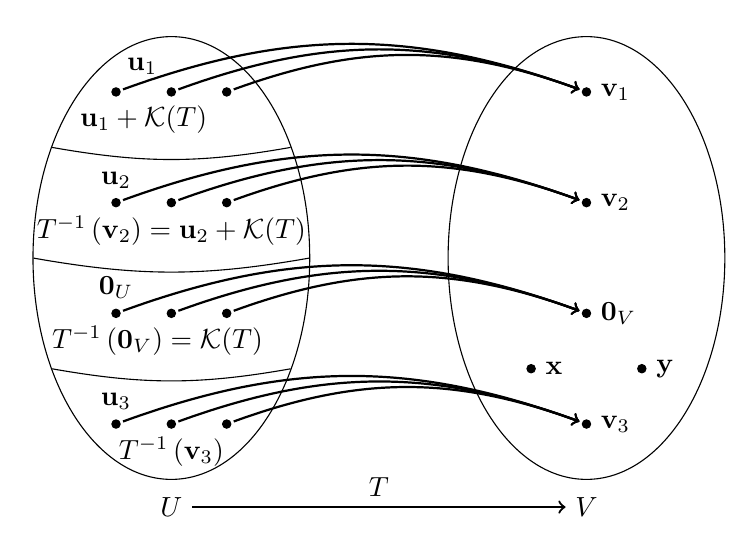
\begin{tikzpicture}
\tikzset{ltvect/.style={shape=circle, minimum size=0.30em, inner sep=0pt, draw, fill=black}}
\tikzset{ltedge/.style={->, bend left=20, thick, shorten <=0.1em, shorten >=0.1em}}
% base generic picture
\draw ( 5em, 8em) circle [x radius=5em, y radius=8em, thick];
\draw (20em, 8em) circle [x radius=5em, y radius=8em, thick];
\node (U) at ( 5em, -1em) {$U$};
\node (V) at (20em, -1em) {$V$};
\draw[->, thick, draw] (U) to node[auto] {$T$} (V);
% inputs
% fine-tune u_1 to fit
\node (u11)    [ltvect, label={[label distance=0.1em]80:$\vect{u}_1$}] at (3em, 14em) {};
\node (u12)    [ltvect]                              at (5em, 14em) {};
\node (u13)    [ltvect]                              at (7em, 14em) {};
\node (u21)    [ltvect, label=above:$\vect{u}_2$]    at (3em, 10em) {};
\node (u22)    [ltvect]                              at (5em, 10em) {};
\node (u23)    [ltvect]                              at (7em, 10em) {};
\node (zeroU1) [ltvect, label=above:$\zerovector_U$] at (3em,  6em) {};
\node (zeroU2) [ltvect]                              at (5em,  6em) {};
\node (zeroU3) [ltvect]                              at (7em,  6em) {};
\node (u31)    [ltvect, label=above:$\vect{u}_3$]    at (3em,  2em) {};
\node (u32)    [ltvect]                              at (5em,  2em) {};
\node (u33)    [ltvect]                              at (7em,  2em) {};
% outputs
\node (v1)    [ltvect, label=right:$\vect{v}_1$]     at (20em, 14em) {};
\node (v2)    [ltvect, label=right:$\vect{v}_2$]     at (20em, 10em) {};
\node (zeroV) [ltvect, label=right:$\zerovector_V$]  at (20em,  6em) {};
\node (o1)    [ltvect, label=right:$\vect{x}$]       at (18em, 4em) {};
\node (o2)    [ltvect, label=right:$\vect{y}$]       at (22em, 4em) {};
\node (v3)    [ltvect, label=right:$\vect{v}_3$]     at (20em,  2em) {};
% associations
\draw[ltedge] (u11) to (v1);
\draw[ltedge] (u12) to (v1);
\draw[ltedge] (u13) to (v1);
\draw[ltedge] (u21) to (v2);
\draw[ltedge] (u22) to (v2);
\draw[ltedge] (u23) to (v2);
\draw[ltedge] (zeroU1) to (zeroV);
\draw[ltedge] (zeroU2) to (zeroV);
\draw[ltedge] (zeroU3) to (zeroV);
\draw[ltedge] (u31) to (v3);
\draw[ltedge] (u32) to (v3);
\draw[ltedge] (u33) to (v3);
% preimages
\node (pre1) at (4em,   13em) {$\vect{u}_1 + \krn{T}$};
\node (pre2) at (5em,    9em) {$\preimage{T}{\vect{v}_2}=\vect{u}_2 + \krn{T}$};
\node (pre3) at (4.5em,  5em) {$\preimage{T}{\zerovector_V}=\krn{T}$};
\node (pre4) at (5em,    1em) {$\preimage{T}{\vect{v}_3}$};
% banding, x-coordinates are +/- 5*sqrt(3)/2 off midline
\node (b11) [minimum size=0em, inner sep=0pt] at (0.669873em, 12em) {};
\node (b12) [minimum size=0em, inner sep=0pt] at (9.330127em, 12em) {};
\node (b21) [minimum size=0em, inner sep=0pt] at (       0em,  8em) {};
\node (b22) [minimum size=0em, inner sep=0pt] at (      10em,  8em) {};
\node (b31) [minimum size=0em, inner sep=0pt] at (0.669873em,  4em) {};
\node (b32) [minimum size=0em, inner sep=0pt] at (9.330127em,  4em) {};
\draw [-, bend right=10] (b11) to (b12);
\draw [-, bend right=10] (b21) to (b22);
\draw [-, bend right=10] (b31) to (b32);
\end{tikzpicture}
\end{image}

The next theorem is one we will cite frequently, as it characterizes injections by the size of the kernel.


\begin{theorem}[Kernel of an Injective Linear Transformation]
\label{theorem:KILT}


Suppose that $\ltdefn{T}{U}{V}$ is a linear transformation.  Then $T$ is injective if and only if the kernel of $T$ is trivial, $\krn{T}=\set{\zerovector}$.




\begin{proof}
($\Rightarrow$) We assume $T$ is injective and we need to establish that two sets are equal (\ref{definition:SE}).  Since the kernel is a subspace (\ref{theorem:KLTS}), $\set{\zerovector}\subseteq\krn{T}$.  To establish the opposite inclusion, suppose $\vect{x}\in\krn{T}$.
\begin{align*}
\lteval{T}{\vect{x}}
&=\zerovector&&\ref{definition:KLT}\\
&=\lteval{T}{\zerovector}
&&\ref{theorem:LTTZZ}
\end{align*}




We can apply \ref{definition:ILT} to conclude that $\vect{x}=\zerovector$.  Therefore $\krn{T}\subseteq\set{\zerovector}$ and by \ref{definition:SE}, $\krn{T}=\set{\zerovector}$.



($\Leftarrow$)  To establish that $T$ is injective, appeal to \ref{definition:ILT} and begin with the assumption that $\lteval{T}{\vect{x}}=\lteval{T}{\vect{y}}$.  Then
\begin{align*}
\lteval{T}{\vect{x}-\vect{y}}
&=\lteval{T}{\vect{x}}-\lteval{T}{\vect{y}}
&&\ref{definition:LT}\\
&=\zerovector
&&\text{Hypothesis}
\end{align*}




So $\vect{x}-\vect{y}\in\krn{T}$ by \ref{definition:KLT} and with the hypothesis that the kernel is trivial we conclude that $\vect{x}-\vect{y}=\zerovector$.  Then
\begin{align*}
\vect{y}
=\vect{y}+\zerovector
=\vect{y}+\left(\vect{x}-\vect{y}\right)
=\vect{x}
\end{align*}
thus establishing that $T$ is injective by \ref{definition:ILT}.



\end{proof}
\end{theorem}

You might begin to think about how \ref{diagram:KPI} would change if the linear transformation is injective, which would make the kernel trivial by \ref{theorem:KILT}.


\begin{example}

Consider (again) the linear transformation
\[
\ltdefn{T}{\complex{5}}{\complex{5}},\quad
\lteval{T}{\colvector{x_1\\x_2\\x_3\\x_4\\x_5}}=
\colvector{-2 x_1 + 3 x_2 + 3 x_3 - 6 x_4 + 3 x_5\\
-16 x_1 + 9 x_2 + 12 x_3 - 28 x_4 + 28 x_5\\
-19 x_1 + 7 x_2 + 14 x_3 - 32 x_4 + 37 x_5\\
-21 x_1 + 9 x_2 + 15 x_3 - 35 x_4 + 39 x_5\\
-9 x_1 + 5 x_2 + 7 x_3 - 16 x_4 + 16 x_5}
\]

Notice that for
\begin{align*}
\vect{x}&=\colvector{1\\3\\-1\\2\\4}&
\vect{y}&=\colvector{4\\7\\0\\5\\7}
\end{align*}
so we have
\begin{align*}
\lteval{T}{\colvector{1\\3\\-1\\2\\4}}&=\colvector{4\\55\\72\\77\\31}&
\lteval{T}{\colvector{4\\7\\0\\5\\7}}&=\colvector{4\\55\\72\\77\\31}
\end{align*}
But just where did those two vectors come from?

The key is the vector
\[
\vect{z}=\colvector{3\\4\\1\\3\\3}
\]
which you can check is an element of $\krn{T}$.  Choose a vector $\vect{x}$ at random, and then compute $\vect{y}=\vect{x}+\vect{z}$ (verify this computation).  Then
\begin{align*}
\lteval{T}{\vect{y}}&=\lteval{T}{\vect{x}+\vect{z}}\\
&=\lteval{T}{\vect{x}}+\lteval{T}{\vect{z}}&&\ref{definition:LT}\\
&=\lteval{T}{\vect{x}}+\zerovector&&\vect{z}\in\krn{T}\\
&=\lteval{T}{\vect{x}}&&\ref{property:Z}
\end{align*}

Whenever the kernel of a linear transformation is nontrivial, we can employ this device and conclude that the linear transformation is not injective.  This is another way of viewing \ref{theorem:KILT}.  For an injective linear transformation, the kernel is trivial and our only choice for $\vect{z}$ is the zero vector, which will not help us create two \textit{different} inputs for $T$ that yield identical outputs.  For every one of the archetypes that is not injective, there is an example presented of exactly this form.

\end{example}

\end{document}
